\hypertarget{creating-tree-graph}{%
\paragraph{\texorpdfstring{Creating tree graph\\
}{Creating tree graph }}\label{creating-tree-graph}}

The first step is to create a directed graph representing the NCBI
Taxonomy tree.

\begin{Shaded}
\begin{Highlighting}[]
\NormalTok{knitr}\OperatorTok{::}\NormalTok{opts_chunk}\OperatorTok{$}\KeywordTok{set}\NormalTok{(}
  \DataTypeTok{warning     =} \OtherTok{FALSE}\NormalTok{,}
  \DataTypeTok{message     =} \OtherTok{FALSE}\NormalTok{,}
  \DataTypeTok{cache       =}\NormalTok{ TRUE}\CommentTok{#,}
  \CommentTok{# cache.path  = "aaaa" }
\NormalTok{)}

\KeywordTok{library}\NormalTok{(here)}
\end{Highlighting}
\end{Shaded}

\begin{verbatim}
## here() starts at C:/R/neuro
\end{verbatim}

\begin{Shaded}
\begin{Highlighting}[]
\KeywordTok{library}\NormalTok{(purrr)}
\KeywordTok{library}\NormalTok{(tibble)}

\KeywordTok{library}\NormalTok{(knitr)}
\KeywordTok{library}\NormalTok{(kableExtra)}

\KeywordTok{library}\NormalTok{(neurotransmissionevolution)}

\CommentTok{# download_if_missing <- function(filename, url) \{}
\CommentTok{#   if (!file.exists(here("data-raw", "download", filename))) \{}
\CommentTok{#     download.file(url, filename)}
\CommentTok{#   \}}
\CommentTok{# \}}

\CommentTok{# files <- tribble(}
\CommentTok{#   ~filename,           ~url,}
\CommentTok{#   "species.v11.0.txt", "https://stringdb-static.org/download/species.v11.0.txt",}
\CommentTok{#   # "download/taxonomy", "https://ftp.ncbi.nlm.nih.gov/pub/taxonomy/new_taxdump/new_taxdump.tar.gz",}
\CommentTok{#   # "x",                 "y",}
\CommentTok{#   # "x",                 "y",}
\CommentTok{# )}

\NormalTok{files <-}\StringTok{ }\KeywordTok{tribble}\NormalTok{(}
  \OperatorTok{~}\NormalTok{url,}
  \OperatorTok{~}\NormalTok{filename,}
  
  \StringTok{"https://stringdb-static.org/download/species.v11.0.txt"}\NormalTok{,}
  \StringTok{"species.v11.0.txt"}\NormalTok{,}
  
  \StringTok{"https://ftp.ncbi.nlm.nih.gov/pub/taxonomy/new_taxdump/new_taxdump.tar.gz"}\NormalTok{,}
  \StringTok{"new_taxdump.tar.gz"}\NormalTok{,}
  
  \StringTok{"http://rest.kegg.jp/link/pathway/hsa"}\NormalTok{,}
  \StringTok{"link_pathway_entrez.tsv"}\NormalTok{,}
  
  \StringTok{"https://string-db.org/mapping_files/entrez/human.entrez_2_string.2018.tsv.gz"}\NormalTok{,}
  \StringTok{"human.entrez_2_string.2018.tsv.gz"}\NormalTok{,}
  
  \StringTok{"https://string-db.org/mapping_files/STRING_display_names/human.name_2_string.tsv.gz"}\NormalTok{,}
  \StringTok{"human.name_2_string.tsv.gz"}\NormalTok{,}
  
  \StringTok{"https://ftp.ncbi.nlm.nih.gov/gene/DATA/GENE_INFO/Mammalia/Homo_sapiens.gene_info.gz"}\NormalTok{,}
  \StringTok{"Homo_sapiens.gene_info.gz"}\NormalTok{,}
  
  \StringTok{"http://rest.genome.jp/link/ensembl/hsa"}\NormalTok{,}
  \StringTok{"link_ensembl_entrez.tsv"}\NormalTok{,}
  
  \CommentTok{# "https://ftp.ncbi.nlm.nih.gov/gene/DATA/GENE_INFO/Mammalia/Homo_sapiens.gene_info.gz",}
  \CommentTok{# "Homo_sapiens.gene_info.gz",}
\NormalTok{)}

\CommentTok{# files %>%}
\CommentTok{#   kable(format = "html") %>%}
\CommentTok{#   kable_styling(bootstrap_options = "striped")}

\NormalTok{files }\OperatorTok
\StringTok{  }\KeywordTok{kable}\NormalTok{(}\StringTok{"latex"}\NormalTok{, }\DataTypeTok{booktabs =}\NormalTok{ T) }\OperatorTok
\StringTok{  }\KeywordTok{kable_styling}\NormalTok{(}\DataTypeTok{latex_options =} \KeywordTok{c}\NormalTok{(}\StringTok{"striped"}\NormalTok{, }\StringTok{"scale_down"}\NormalTok{))}
\end{Highlighting}
\end{Shaded}

\begin{table}[H]
\centering
\resizebox{\linewidth}{!}{
\begin{tabular}{ll}
\toprule
url & filename\\
\midrule
\rowcolor{gray!6}  https://stringdb-static.org/download/species.v11.0.txt & species.v11.0.txt\\
https://ftp.ncbi.nlm.nih.gov/pub/taxonomy/new\_taxdump/new\_taxdump.tar.gz & new\_taxdump.tar.gz\\
\rowcolor{gray!6}  http://rest.kegg.jp/link/pathway/hsa & link\_pathway\_entrez.tsv\\
https://string-db.org/mapping\_files/entrez/human.entrez\_2\_string.2018.tsv.gz & human.entrez\_2\_string.2018.tsv.gz\\
\rowcolor{gray!6}  https://string-db.org/mapping\_files/STRING\_display\_names/human.name\_2\_string.tsv.gz & human.name\_2\_string.tsv.gz\\
\addlinespace
https://ftp.ncbi.nlm.nih.gov/gene/DATA/GENE\_INFO/Mammalia/Homo\_sapiens.gene\_info.gz & Homo\_sapiens.gene\_info.gz\\
\rowcolor{gray!6}  http://rest.genome.jp/link/ensembl/hsa & link\_ensembl\_entrez.tsv\\
\bottomrule
\end{tabular}}
\end{table}

\begin{itemize}
\tightlist
\item
  \textbf{test\_table.tsv}

  \begin{itemize}
  \tightlist
  \item
    Just testing description
  \end{itemize}

  \begin{enumerate}
  \def\labelenumi{\arabic{enumi}.}
  \tightlist
  \item
    \textbf{string\_id}
  \end{enumerate}

  \begin{itemize}
  \tightlist
  \item
    \textbf{Description:} This represents the string protein identifier
  \item
    \textbf{Type:} numeric
  \item
    \textbf{Used:} yes
  \item
    \textbf{Example:} 9606.ENSP000007157
  \end{itemize}

  \begin{enumerate}
  \def\labelenumi{\arabic{enumi}.}
  \setcounter{enumi}{1}
  \tightlist
  \item
    \textbf{length}
  \end{enumerate}

  \begin{itemize}
  \tightlist
  \item
    \textbf{Description:} This represents the protein size
  \item
    \textbf{Type:} numeric
  \item
    \textbf{Used:} no
  \item
    \textbf{Example:} 462
  \end{itemize}
\end{itemize}

First table

\begin{Shaded}
\begin{Highlighting}[]
\NormalTok{spec <-}\StringTok{ }\NormalTok{tibble}\OperatorTok{::}\KeywordTok{tribble}\NormalTok{(}
  \OperatorTok{~}\NormalTok{col_name, }\OperatorTok{~}\NormalTok{col_type, }\OperatorTok{~}\NormalTok{used, }\OperatorTok{~}\NormalTok{ex, }\OperatorTok{~}\NormalTok{desc,}
  \StringTok{"string_id"}\NormalTok{, }\StringTok{"numeric"}\NormalTok{, }\StringTok{"yes"}\NormalTok{, }\StringTok{"9606.ENSP000007157"}\NormalTok{, }\KeywordTok{paste}\NormalTok{(}\StringTok{"This represents the string protein identifier."}\NormalTok{,}
                                                             \StringTok{"Like, really cool! Lorem ipsum dolar sit amet."}\NormalTok{,}
                                                             \StringTok{"Niiiiii. Lero lero coronavirus coronaipsum."}\NormalTok{),}
  \StringTok{"length"}\NormalTok{, }\StringTok{"numeric"}\NormalTok{, }\StringTok{"no"}\NormalTok{, }\StringTok{"462"}\NormalTok{, }\StringTok{"This represents the protein size"}\NormalTok{,}
\NormalTok{)}

\CommentTok{# spec %>%}
\CommentTok{#   kable("latex", booktabs = T) %>%}
\CommentTok{#   add_header_above(c("test_table.tsv" = ncol(spec))) %>%}
\CommentTok{#   kable_styling(latex_options = c("striped", "scale_down")) %>%}
\CommentTok{#   column_spec(ncol(spec), width = "20em")}
\CommentTok{# print_dataframe_specification(spec, "a", "b", "caption")}
\end{Highlighting}
\end{Shaded}

\begin{Shaded}
\begin{Highlighting}[]
\CommentTok{# pwalk(files, download_if_missing)}
\KeywordTok{plot}\NormalTok{(}\DecValTok{1}\NormalTok{,}\DecValTok{1}\NormalTok{)}
\end{Highlighting}
\end{Shaded}

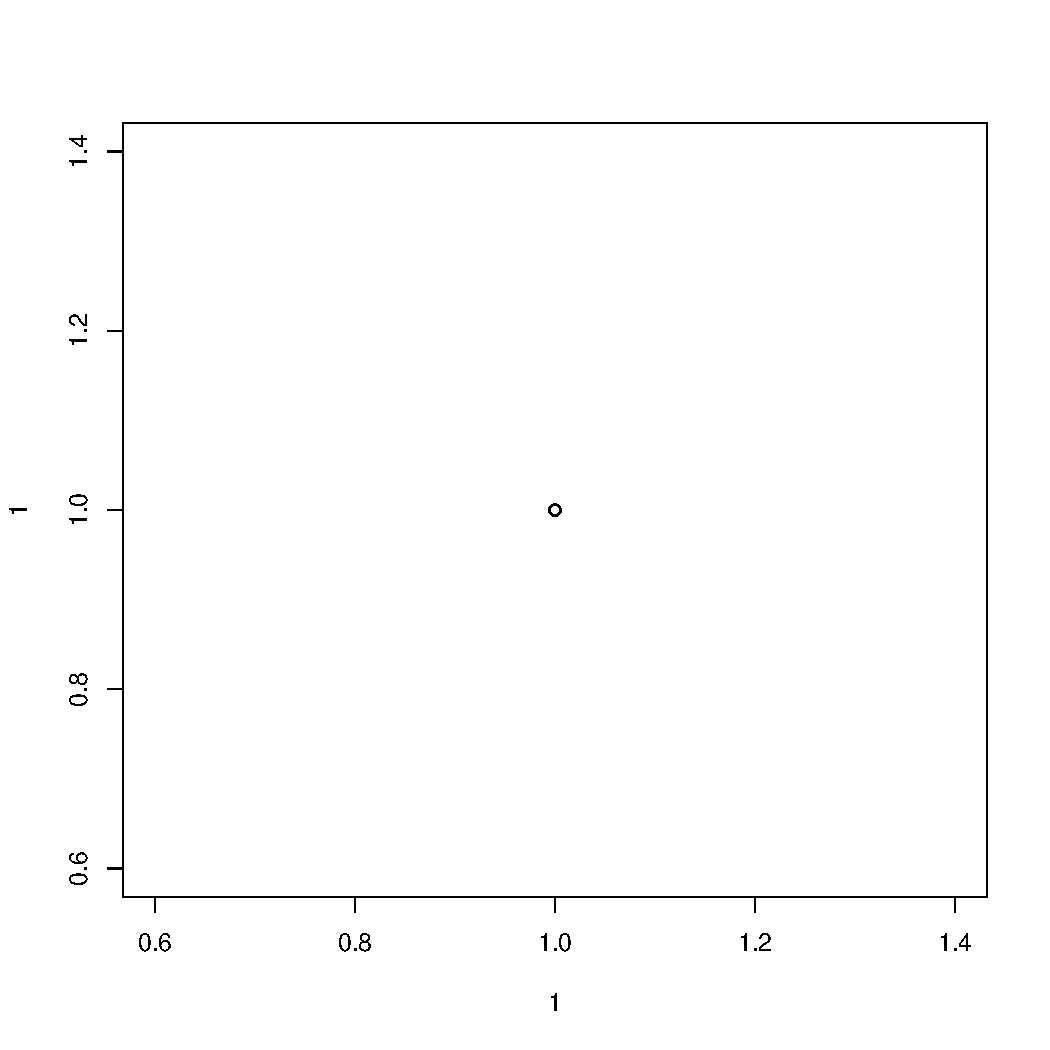
\includegraphics{figs/data-raw.download_files.unnamed-chunk-3-1.pdf}

\begin{Shaded}
\begin{Highlighting}[]
\CommentTok{# barplot(1:3)}
\CommentTok{# dev.copy(pdf, "knit_copy.pdf")}
\CommentTok{# dev.print(pdf, "knit_print.pdf")}
\CommentTok{# print_dataframe_specification(spec, "a", "b", "caption")}
\KeywordTok{kable}\NormalTok{(spec)}
\end{Highlighting}
\end{Shaded}

